\documentclass[%
 reprint,
%superscriptaddress,
%groupedaddress,
%unsortedaddress,
%runinaddress,
%frontmatterverbose, 
%preprint,
%preprintnumbers,
%nofootinbib,
%nobibnotes,
%bibnotes,
 amsmath,amssymb,
 aps,
%pra,
prb,
%rmp,
%prstab,
%prstper,
floatfix,
]{revtex4-2}

\usepackage{graphicx}% Include figure files
\usepackage{dcolumn}% Align table columns on decimal point
\usepackage{bm}% bold math
\usepackage{hyperref}% add hypertext capabilities
\hypersetup{colorlinks=true,urlcolor={blue},citecolor={blue}, linkcolor={blue}}
\usepackage{amsmath} % or simply amstext
%\newcommand{\angstrom}{\textup{\angstrom}}
\usepackage{siunitx}
\usepackage{color}
\usepackage[normalem]{ulem}
\usepackage{diagbox}
\usepackage{import}
\usepackage{multirow}
\usepackage{xr} % referencing across multiple files
\usepackage{cleveref} % cite figures in SI

%\usepackage{url}            % simple URL typesetting
%\usepackage[mathlines]{lineno}% Enable numbering of text and display math
%\linenumbers\relax % Commence numbering lines
%\usepackage{nameref}

%\usepackage[showframe,%Uncomment any one of the following lines to test 
%%scale=0.7, marginratio={1:1, 2:3}, ignoreall,% default settings
%%text={7in,10in},centering,
%%margin=1.5in,
%%total={6.5in,8.75in}, top=1.2in, left=0.9in, includefoot,
%%height=10in,a5paper,hmargin={3cm,0.8in},
%]{geometry}

%RZK: do not edit red text
\newcommand{\lock}{\color{red}}

\renewcommand{\figurename}{Supporting Figure}
\renewcommand{\tablename}{Supporting Table}
\renewcommand{\thefigure}{S\arabic{figure}}
\renewcommand{\thetable}{S\arabic{table}}

\begin{document}

\title{Supporting Information for \\
RZK0422: Add title when the manuscript is ready}% Force line breaks with \\
%\thanks{A footnote to the article title}%

\author{Zhenzhe Zhang}
\author{Dmitrii F. Perepichka}%
\email{dmitrii.perepichka@mcgill.ca}
\author{Rustam Z. Khaliullin}
\email{rustam.khaliullin@mcgill.ca}
\affiliation{%
 Department of Chemistry, McGill University, 801 Sherbrooke St West, Montreal, QC H3A 0B8, Canada
 %This line break forced with \textbackslash\textbackslash
}%

%\date{\today}% It is always \today, today,
             %  but any date may be explicitly specified

\maketitle

The mechanism of classical Ullmann coupling is relatively well understood (Fig.~\ref{fig:classical}).
%The Ullmann coupling reactions discussed above occur mostly in organic solvents. 
It is widely accepted that an aryl halides molecule reacts with Cu species to form an organometallic intermediate. 
This intermediate then reacts with a second aryl molecule through oxidative addition producing a diaryl organomitallic intermediate, which subsequently undergoes reductive elimination to form a covalent bond between the two aryls.

\begin{figure}[htb]
\centering
\includegraphics[width=1.0\columnwidth]{Fig/ullmann_mechanism.png}
\caption{Mechanism of the Ullmann coupling reaction. SET stands for single-electron transfer.
}
\label{fig:classical}
\end{figure}


\textbf{Formation of organometallic intermediates on the Cu(111) surface.} Organic precursors are physisorbed on a metal surface before undergoing chemical transformations. Although the binding of chlorobenzene, bromobenzene and iodobenzene to Cu(111) calculated in this work is stronger than that obtained previously using the a different XC functional~\cite{jacs2013} the trends in the physisorption energies for different halogens are almost exactly the same (Table~\ref{table:bondlength}).

\newpage

\begin{table*}
\centering
\begin{tabular}{ lcccccccc  }
 \hline
 \hline
 Distance & Hal. & \textbf{PHYS} & \textbf{DHAL$\ddagger$} & $\Delta$ (\textbf{DHAL$\ddagger$}$-$\textbf{PHYS}) & \textbf{DHAL} & $\Delta$ (\textbf{DHAL}$-$\textbf{PHYS}) & \textbf{DHAL-2}& \textbf{CMC} \\ 
 \hline 
 \multirow{3}{*}{C--Hal (\si{\angstrom})} & Cl & 1.74 & 2.18 & +0.44 & 3.99 & +2.25 & & \\ 
 %\cline{2-5}
 & Br & 1.91 & 2.46 & +0.55 & 4.10 &+2.19 & & \\ 
 %\cline{2-5}
 & I & 2.12 & 2.61 & +0.49 & 5.10 &+2.98 & & \\ 
 %\cline{2-5}
 \hline
 \multirow{3}{*}{C--Cu (\si{\angstrom}) } & Cl & 3.54 & 2.52 & -1.02 & 2.01 & -1.53 & & \\ 
 & Br & 3.40 & 2.77 & -0.63 & 2.01 & -1.39 & & \\ 
 & I &3.42 & 2.73 &-0.69 & 2.01 & -1.41 & & \\ 
 \hline
 \multirow{3}{*}{Hal--Cu (\si{\angstrom}) } & Cl & 2.99 & 2.37 & -0.62 & 3.50 & +0.51 & &\\ 
 & Br & 2.89 & 2.50 & -0.49 & 3.57 & +0.68 & & \\ 
 & I &2.80 & 2.64 &-0.16 & 3.74 & +0.94 & & \\ 
 \hline
 \hline
 Energy & & & & Barrier & & Change & & \\
 \hline
 \multirow{3}{*}{E (\si{\electronvolt}) } & Cl & -1.07 & 0.17 & 1.24 (+0.35) &-1.65 & -0.58 (+0.23) &-3.30 &-3.05 \\ 
 & Br &-1.14 &-0.25 & 0.89 & -1.95& -0.81 &-3.90 &-3.73\\ 
 & I  & -1.32 & -0.69 & 0.63 (-0.26) & -2.28& -0.96 (-0.15) &-4.55 & -4.38\\ 
 \hline
 \multirow{2}{*}{E (\si{\electronvolt})~\cite{jacs2013}} & Br &-0.95 & & 0.66 & & -0.68 & & \\ 
 & I & -1.12 & & 0.40 (-0.26) & & -0.81 (-0.12) & & \\ 
 \hline
 \hline
\end{tabular}
\caption{Geometric and energetic characterization of the early steps of the Ullmann reaction. Values in parentheses are properties relative to those of bromine-containing states. RZK0603: Add DHAL-2 and CMC states here.}
\label{table:bondlength}
\end{table*}
%ZZ0628: The geometry of DHAL-2 state is the same as DHAL, and CMC has been reported in main text.

\newpage



\begin{figure*}[h!]
\centering
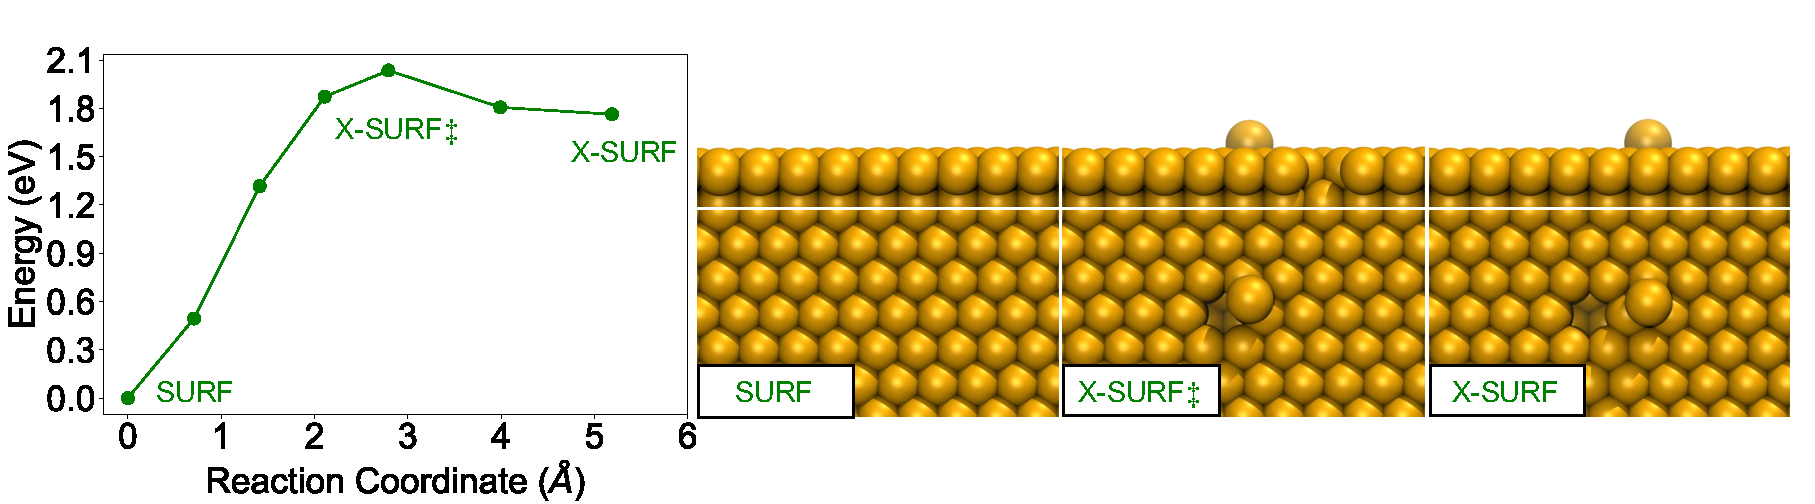
\includegraphics[width=1.0\textwidth]{Fig/pureadatomform.pdf}
\caption{Energetics of an adatom formation on the clean Cu(111) surface.}
\label{fig:cleanatomform}
\end{figure*}

\begin{figure*}[hbt]
\centering
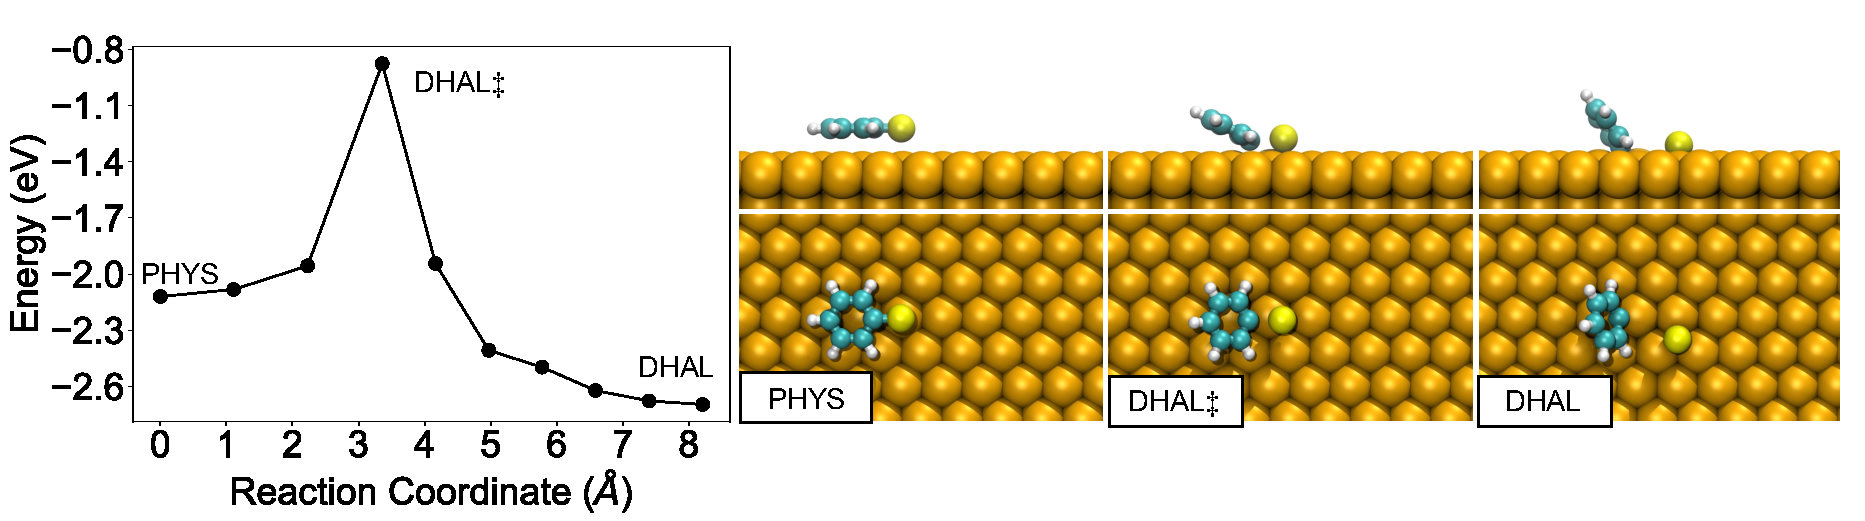
\includegraphics[width=1.0\textwidth]{Fig/dissociation_Cl.pdf}
\caption{The dissociation of C-Cl bond on Cu(111) surface. Left is the energy diagram of the CI-NEB calculations, right side are the top and side views of geometry of $IS$, $TS$ and $FS$. (Sphere with ochre color is copper atoms, with cyan color is carbon atoms, with white color is hydrogen atoms, sphere with yellow color is chlorine atom)}
\label{fig:dissociation_Cl}
\end{figure*}



\begin{figure*}[hbt]
\centering
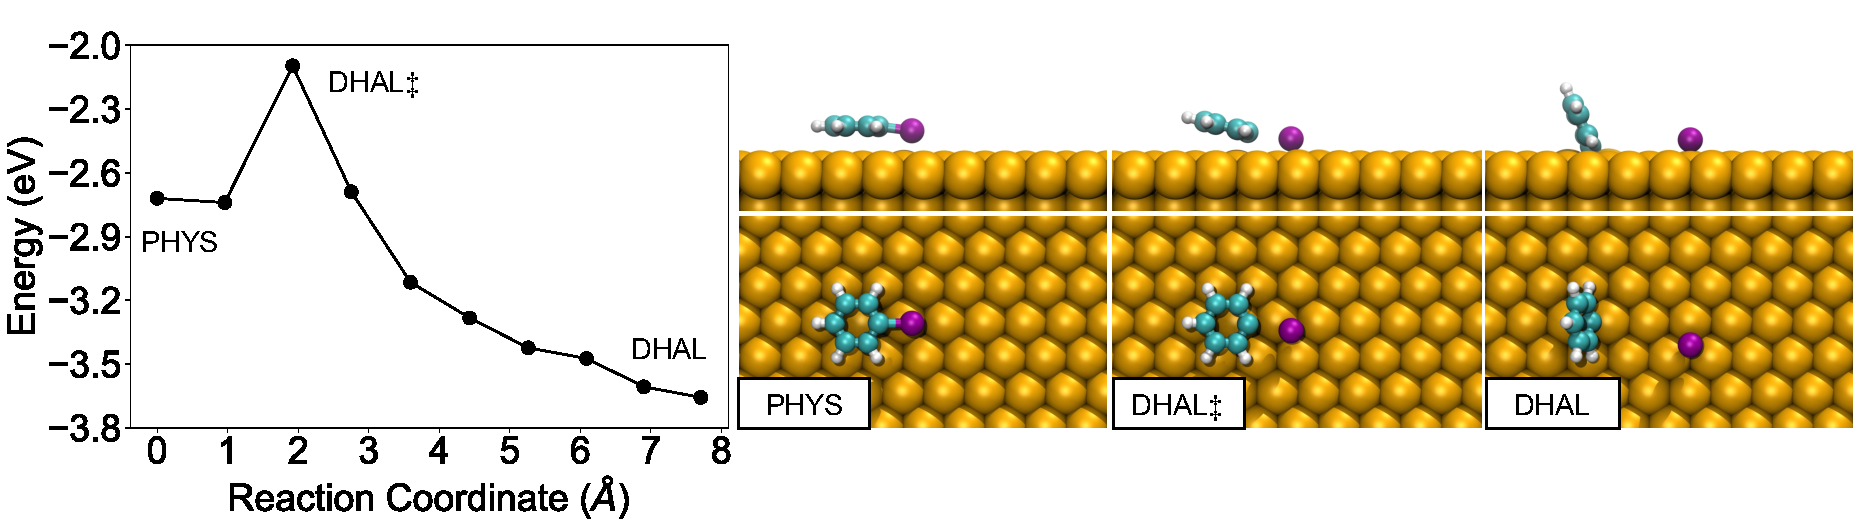
\includegraphics[width=1.0\textwidth]{Fig/dissociation_I.pdf}
\caption{The dissociation of C-I bond on Cu(111) surface. Left is the energy diagram of the CI-NEB calculations, right side are the top and side views of geometry of $IS$, $TS$ and $FS$. (Sphere with ochre color is copper atom, with cyan color is carbon atom, with white color is hydrogen atom, sphere with red color is iodine atoms)}
\label{fig:dissociation_I}
\end{figure*}

\begin{figure}[hbt]
\centering
\includegraphics[width=0.45\textwidth]{Fig/FormingC-Cu-C.pdf}
\caption{RZK0415: This figure is now obsolete and must be removed. It does not report any info complementary to the main energy profile.
Energy diagram of forming C--Cu--C bridge intermediates structures from dechlorinated, debrominated and deiodinated benzene. The energy is computed as the difference between 2 $\times$ dehalogenated intermediates (left geometry) and C--Cu--C bridge intermediate structure $+$ two bromine atoms on Cu(111) surface. The blue circles represent chlorine, bromine or iodine atoms respectively in three situations. Yellow line with circle points is dechlorinated benzene to C--Cu--C, pink line with square points is debrominated benzene to C--Cu--C and red line with triangle points is deiodinated benzene to C--Cu--C.}
\label{fig:formingBridge}
\end{figure}

\begin{table*}
\centering
\begin{tabular}{ lccccccccccccc  }
 \hline
 \hline
 Distance & Halogen & \textbf{CMC}$^{a}$ & \textbf{X-CMC$\ddagger$}$^{b}$ & $\Delta (b-a)$ & \textbf{X-CMC}$^{c}$ &$\Delta (c-a)$ & \textbf{X-DIM$\ddagger$}$^{d}$ & $\Delta (d-c)$ & \textbf{X-DIM-A}$^{e}$ &$\Delta (e-c)$ & \textbf{X-DIM-B}  \\ 
 \hline 
 \multirow{3}{*}{C--C (\si{\angstrom})} & Cl & \multirow{3}{*}{3.10} & \multirow{3}{*}{3.55} & \multirow{3}{*}{+0.45} & \multirow{3}{*}{3.89} &\multirow{3}{*}{+0.79} & \multirow{3}{*}{2.53} &\multirow{3}{*}{-1.36} & \multirow{3}{*}{1.50} &\multirow{3}{*}{-2.39}\\ 
 & Br & &  &  &  & & & & & &\\ 
 & I & &  &  &  & & & & & &\\ 
 \hline
 \multirow{3}{*}{C--Cu (\si{\angstrom}) } & Cl & \multirow{3}{*}{2.06} & \multirow{3}{*}{1.85} & \multirow{3}{*}{-0.21} & \multirow{3}{*}{1.96} &\multirow{3}{*}{-0.10} & \multirow{3}{*}{1.90} & \multirow{3}{*}{-0.06} & \multirow{3}{*}{2.14} &\multirow{3}{*}{+0.18} &\multirow{3}{*}{} \\ 
 & Br &  &  & & & &  & & & &\\ 
 & I & &  &  & & & & & & & \\ 
 \hline
 \multirow{3}{*}{Cu$_{\rm lift}$ (\si{\angstrom}) } & Cl & \multirow{3}{*}{0.53} & \multirow{3}{*}{1.68} & \multirow{3}{*}{+1.16} & \multirow{3}{*}{2.02} &\multirow{3}{*}{+1.49} & \multirow{3}{*}{1.77} & \multirow{3}{*}{-0.25} & \multirow{3}{*}{1.76} &\multirow{3}{*}{-0.26} &\multirow{3}{*}{0.00}\\ 
 & Br &  &  &  &  & & & &  & &\\ 
 & I & &  &  &  & & & & & &\\ 
 \hline
 \hline
 Energy  & & & & Barrier & & Change & & Barrier & &Change&\\
 \hline
 \multirow{3}{*}{E (\si{\electronvolt}) } & Cl & -3.05 &-1.67 & +1.38 &-3.26 &-0.21 & -1.25 & +2.01& -3.42&-0.16&-3.29\\ 
 & Br &-3.73 &-2.35 &+1.38 & -3.94 &-0.21 & -1.93 & +2.01 & -4.11 & -0.16&-3.97 \\ 
 & I  & -4.38 & -3.00 & +1.38 & -4.59 &-0.21 & -2.58& +2.01 & -4.76 & -0.16&-4.62\\ 
 \hline
 \hline
\end{tabular}
\caption{Geometric and energetic characterization of the C--C coupling step with creation of an adatom along latitude direaction. Energies are reported relative to the \textbf{SURF} state.}
\label{table:adatom-110}
\end{table*}




\bibliographystyle{apsrev4-1} % Tell bibtex which bibliography style to use
\bibliography{references}% Produces the bibliography via BibTeX.

\end{document}








